\subsection{Results}



\begin{table}[t]
\footnotesize
  \caption{Performance over granularity levels relative to $\text{TLO}^A$. Items are significantly different from $\text{TLO}^A$ when marked *$p<0.05$, ** $p <0.01$, *** $p<0.001$.}
  \label{tab:granularity_significance}
\begin{adjustbox}{width=\columnwidth}

\begin{tabular}{>{\raggedright\arraybackslash}p{5em}>{\raggedleft\arraybackslash}p{4em}>{\raggedright\arraybackslash}p{4.5em}rrrr}
\toprule
Environment & RewGranularity & PenGranularity & LIN_SUM & SFLLA1 & EEBA1 & TLO$^A$\\
\midrule
 &  & 0.01 & 1.47*** & 6.61*** & 1.51** & \\

 &  & 1.00 & 1.57** & 4.08*** & 1.46*** & \\

 & \multirow[t]{-3}{4em}{\raggedleft\arraybackslash 0.00} & 100.00 & 1.44*** & 1.39*** & 1.58* & \\
\cmidrule{2-6}
 & 0.01 &  & 1.38*** & 6.47*** & 1.42*** & \\
\cmidrule{2-2}
\cmidrule{4-6}
 & 1.00 &  & 1.46*** & 6.37*** & 1.09*** & \\
\cmidrule{2-2}
\cmidrule{4-6}
\multirow[t]{-6}{5em}{\raggedright\arraybackslash Breakable Bottles} & 100.00 & \multirow[t]{-3}{4.5em}{\raggedright\arraybackslash 0.00} & 1.49** & -40.38*** & -41.39*** & \multirow[t]{-6}{*}{\raggedleft\arraybackslash 1.82}\\
\cmidrule{1-7}
 &  & 0.01 & -0.48*** & 4.02 & 1.50*** & \\

 &  & 1.00 & -0.51*** & 4.64*** & 1.39*** & \\

 & \multirow[t]{-3}{4em}{\raggedleft\arraybackslash 0.00} & 100.00 & -0.45*** & -1.02*** & -1.08*** & \\
\cmidrule{2-6}
 & 0.01 &  & -0.47*** & 3.96 & 0.92*** & \\
\cmidrule{2-2}
\cmidrule{4-6}
 & 1.00 &  & -0.46*** & 3.80 & 1.17*** & \\
\cmidrule{2-2}
\cmidrule{4-6}
\multirow[t]{-6}{5em}{\raggedright\arraybackslash Doors} & 100.00 & \multirow[t]{-3}{4.5em}{\raggedright\arraybackslash 0.00} & -0.38*** & -39.01*** & -41.87*** & \multirow[t]{-6}{*}{\raggedleft\arraybackslash 3.96}\\
\cmidrule{1-7}
 &  & 0.01 & -14.97*** & -10.31*** & -15.01*** & \\

 &  & 1.00 & -14.96*** & -14.90*** & -14.96*** & \\

 & \multirow[t]{-3}{4em}{\raggedleft\arraybackslash 0.00} & 100.00 & -15.05*** & -15.01*** &  & \\
\cmidrule{2-5}
 & 0.01 &  & -15.00*** & -10.83*** & \multirow[t]{-2}{*}{\raggedleft\arraybackslash -14.99***} & \\
\cmidrule{2-2}
\cmidrule{4-6}
 & 1.00 &  & -14.98*** & -7.43*** & -14.86*** & \\
\cmidrule{2-2}
\cmidrule{4-6}
\multirow[t]{-6}{5em}{\raggedright\arraybackslash Sokoban} & 100.00 & \multirow[t]{-3}{4.5em}{\raggedright\arraybackslash 0.00} & -14.96*** & -9.44*** & -10.52*** & \multirow[t]{-6}{*}{\raggedleft\arraybackslash 10.80}\\
\cmidrule{1-7}
 &  & 0.01 & 28.72*** & 27.94*** & 28.73*** & \\

 &  & 1.00 & 28.71*** & 28.77*** & 28.70*** & \\

 & \multirow[t]{-3}{4em}{\raggedleft\arraybackslash 0.00} & 100.00 & 28.77*** & 28.72*** & 28.76*** & \\
\cmidrule{2-6}
 & 0.01 &  & 28.76*** & 27.91*** & 28.73*** & \\
\cmidrule{2-2}
\cmidrule{4-6}
 & 1.00 &  & 28.73*** & 27.79*** & 28.64*** & \\
\cmidrule{2-2}
\cmidrule{4-6}
\multirow[t]{-6}{5em}{\raggedright\arraybackslash Unbreakable Bottles} & 100.00 & \multirow[t]{-3}{4.5em}{\raggedright\arraybackslash 0.00} & 28.74*** & -8.23*** & -13.27*** & \multirow[t]{-6}{*}{\raggedleft\arraybackslash 27.10}\\
\bottomrule
\end{tabular}

\end{adjustbox}
\end{table}


\begin{figure}
  %\centering
  %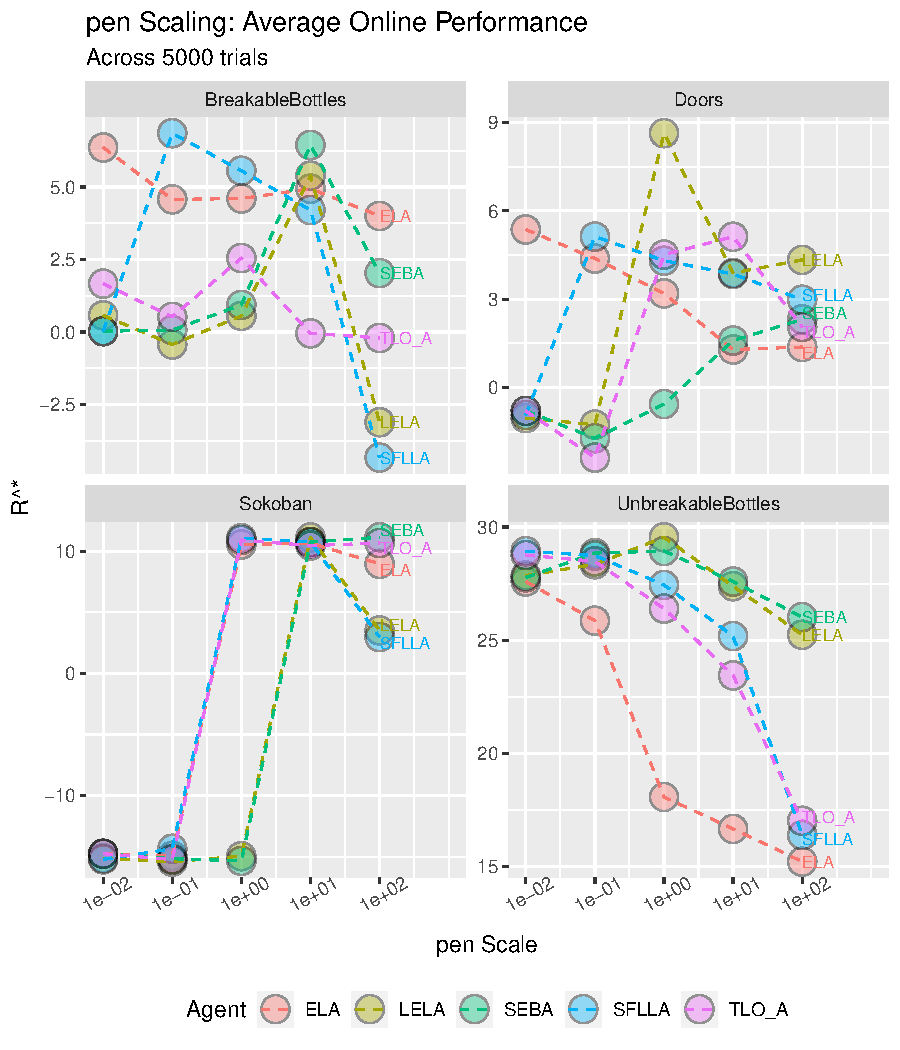
\includegraphics[width=\columnwidth]{output/onlinepen.pdf}
  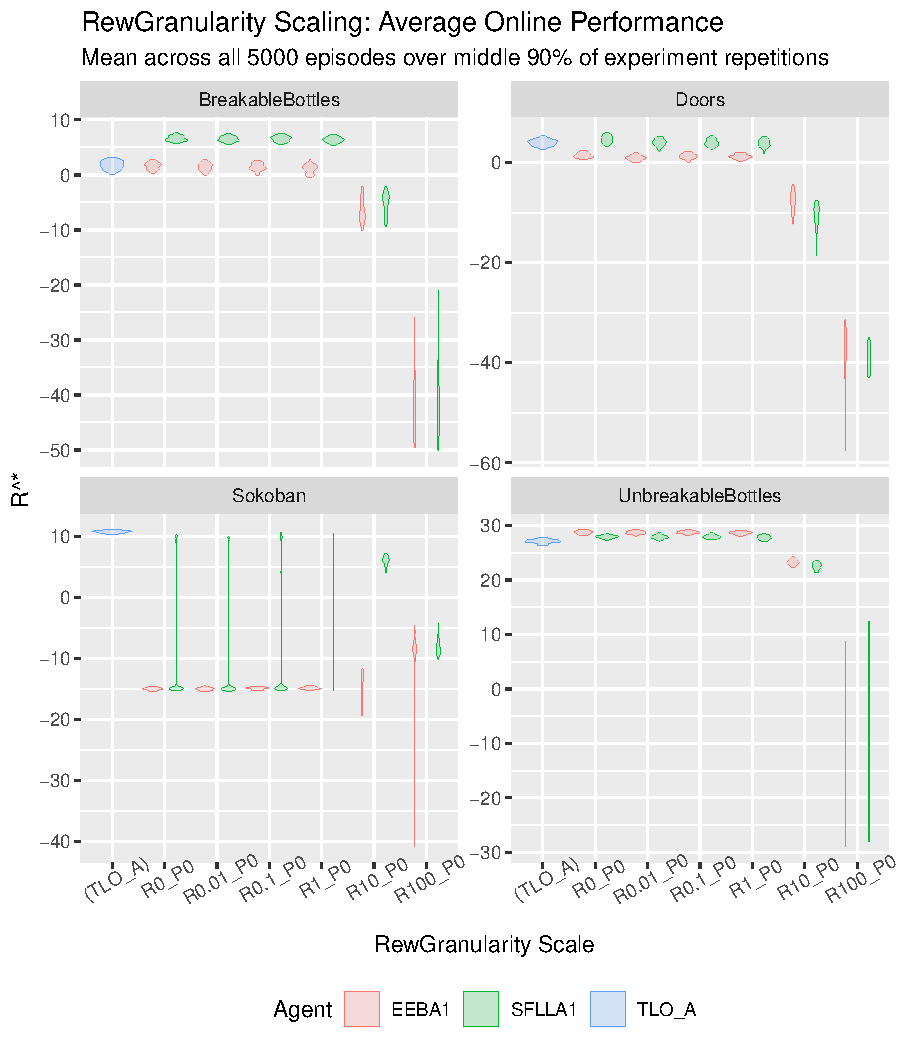
\includegraphics[width=\columnwidth]{output/multirun_n100_pilot_granularityonline_RewGranularity.pdf}
  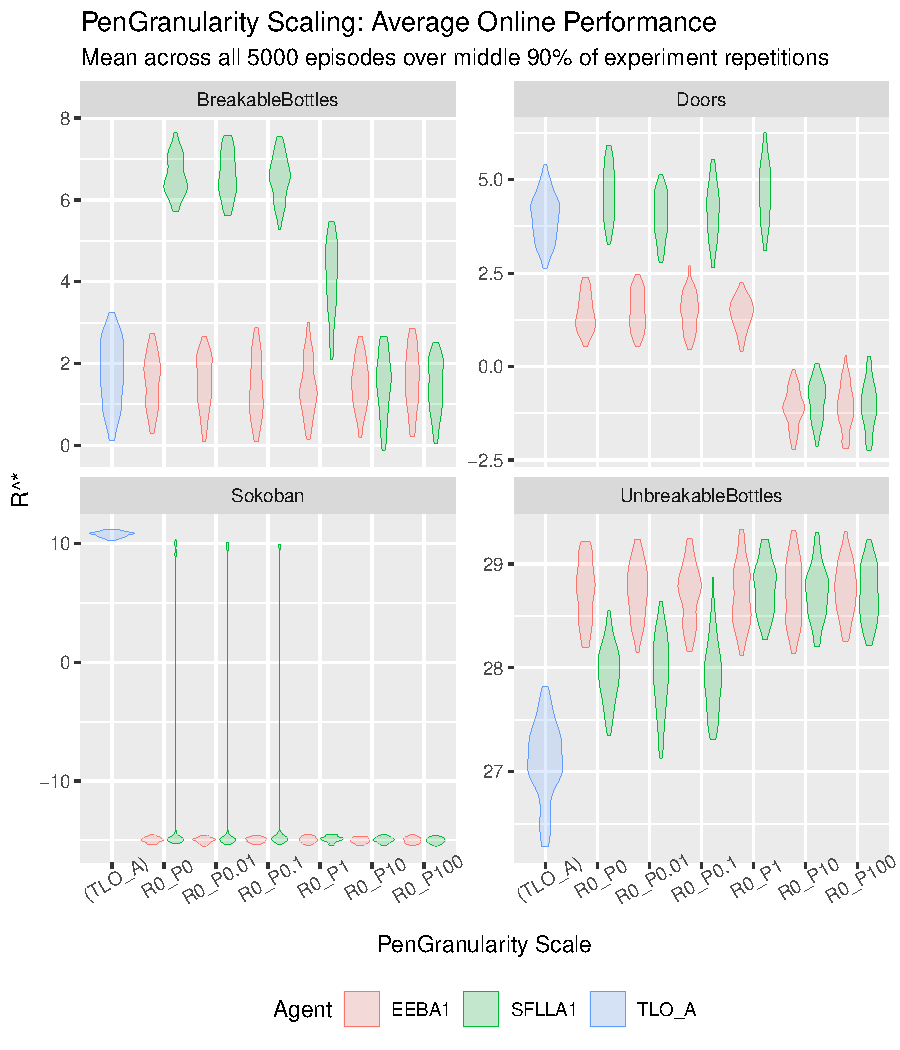
\includegraphics[width=\columnwidth]{output/multirun_n100_pilot_granularityonline_PenGranularity.pdf}
  \caption{By creating `granularity' for our non-linear transform agents, we can simulate similarity with $TLO_A$, which might be considered as a custom-tuned form of granularity.
  }
   \label{fig:exp3_main}
   \Description{By creating `granularity' for our non-linear transform agents, we can simulate similarity with $TLO_A$, which might be considered as a custom-tuned form of granularity.}
 \end{figure}
 
For SFELLA, as expected, performance declined as granularity increased, particularly in the BreakableBottles environment where it previously had a clear advantage over $TLO_A$ (Figure~\ref{fig:exp3_main}). For UnbreakableBottles, performance declined as granularity for the Reward Scaling (???) was increased. In the Doors environment, performance declined, from significantly better (??? Table~\ref{tab:granularity_significance}) than $TLO_A$ to much, much worse. In the Sokoban environment, as in Experiment 1, $TLO_A$ was the better performer and remained so.

The result confirms that where SFELLA performs well, it does so because it avoids `granularity' and is sensitive to changes in reward right across teh scale. In contrast, $TLO_A$ is sometimes insensitive to changes that exceed its threshold. Where it is well tuned, it performs well, or even better, than othere algorithms, but when not well-tunred, it performs less well.



